\documentclass[]{article}

\usepackage{tikz}
\usetikzlibrary{shapes, arrows}
\usepackage{amsmath}
\newcommand{\mx}[1]{\mathbf{\bm{#1}}} % Matrix command
\newcommand{\vc}[1]{\mathbf{\bm{#1}}} % Vector command
\usepackage{geometry}
 \geometry{
 a4paper,
 total={170mm,257mm},
 left=5mm,
 top=10mm,
 }

\begin{document}

% define the layers to draw the diagram
\pgfdeclarelayer{background}
\pgfdeclarelayer{foreground}
\pgfsetlayers{background,main,foreground}

% define block styles used later
\tikzstyle{image} = [inner sep=0pt]
\tikzstyle{label} = [rectangle, align=center, text width=1.5cm, font=\bfseries]

\begin{tikzpicture}[line width=0.5mm, node distance=0pt]
    \pagenumbering{gobble}
    
    \node (c1) [label] {drink};
    \node (i1_1) [image, right of=c1, xshift=0.18\textwidth] {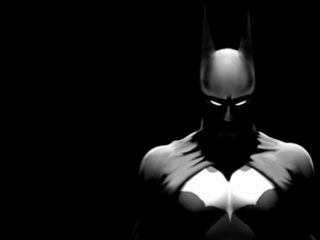
\includegraphics[width=.2\textwidth]{images/img.jpg}};
    \node (i1_2) [image, right of=i1_1, xshift=0.2\textwidth] {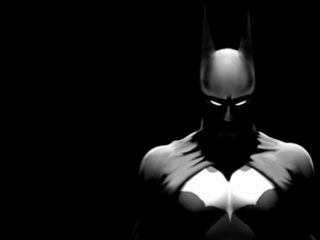
\includegraphics[width=.2\textwidth]{images/img.jpg}};
    \node (i1_3) [image, right of=i1_2, xshift=0.2\textwidth] {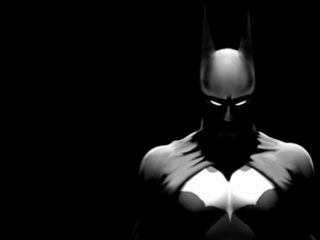
\includegraphics[width=.2\textwidth]{images/img.jpg}};
    \node (i1_4) [image, right of=i1_3, xshift=0.2\textwidth] {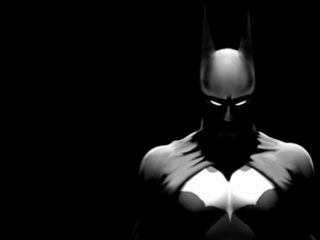
\includegraphics[width=.2\textwidth]{images/img.jpg}};
    \node (i1_5) [image, right of=i1_4, xshift=0.2\textwidth] {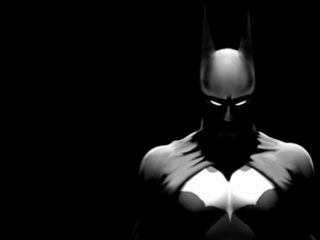
\includegraphics[width=.2\textwidth]{images/img.jpg}};

    \node (c2) [label, below of=c1, yshift=-0.2\textwidth] {eat};
    \node (i2_1) [image, right of=c2, xshift=0.18\textwidth] {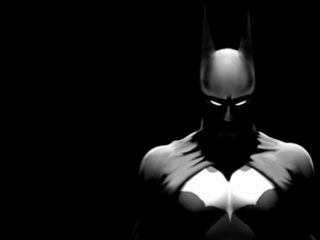
\includegraphics[width=.2\textwidth]{images/img.jpg}};
    \node (i2_2) [image, right of=i2_1, xshift=0.2\textwidth] {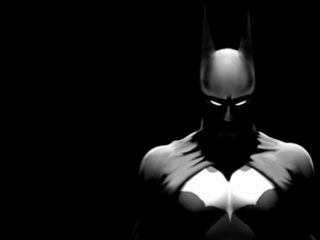
\includegraphics[width=.2\textwidth]{images/img.jpg}};
    \node (i2_3) [image, right of=i2_2, xshift=0.2\textwidth] {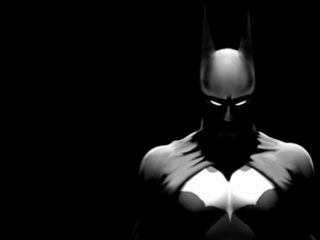
\includegraphics[width=.2\textwidth]{images/img.jpg}};
    \node (i2_4) [image, right of=i2_3, xshift=0.2\textwidth] {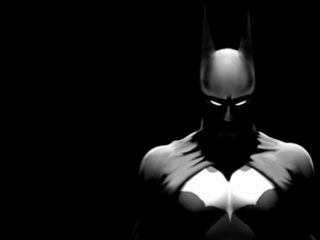
\includegraphics[width=.2\textwidth]{images/img.jpg}};
    \node (i2_5) [image, right of=i2_4, xshift=0.2\textwidth] {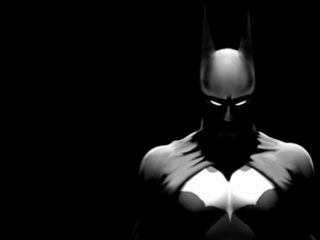
\includegraphics[width=.2\textwidth]{images/img.jpg}};

    \node (c3) [label, below of=c2, yshift=-0.2\textwidth] {groom};
    \node (i3_1) [image, right of=c3, xshift=0.18\textwidth] {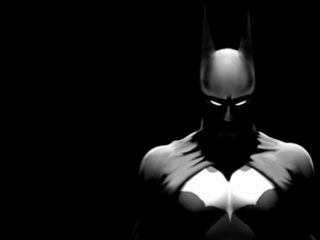
\includegraphics[width=.2\textwidth]{images/img.jpg}};
    \node (i3_2) [image, right of=i3_1, xshift=0.2\textwidth] {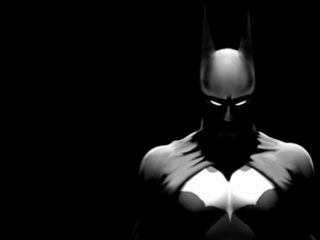
\includegraphics[width=.2\textwidth]{images/img.jpg}};
    \node (i3_3) [image, right of=i3_2, xshift=0.2\textwidth] {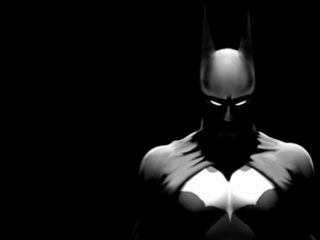
\includegraphics[width=.2\textwidth]{images/img.jpg}};
    \node (i3_4) [image, right of=i3_3, xshift=0.2\textwidth] {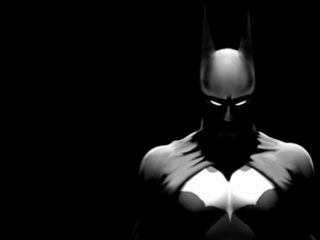
\includegraphics[width=.2\textwidth]{images/img.jpg}};
    \node (i3_5) [image, right of=i3_4, xshift=0.2\textwidth] {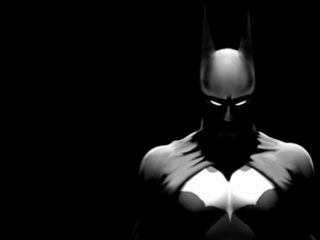
\includegraphics[width=.2\textwidth]{images/img.jpg}};

    \node (c4) [label, below of=c3, yshift=-0.2\textwidth] {hang};
    \node (i4_1) [image, right of=c4, xshift=0.18\textwidth] {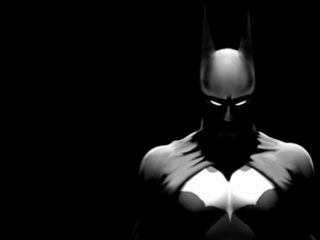
\includegraphics[width=.2\textwidth]{images/img.jpg}};
    \node (i4_2) [image, right of=i4_1, xshift=0.2\textwidth] {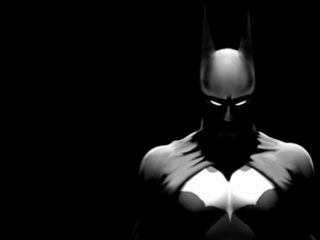
\includegraphics[width=.2\textwidth]{images/img.jpg}};
    \node (i4_3) [image, right of=i4_2, xshift=0.2\textwidth] {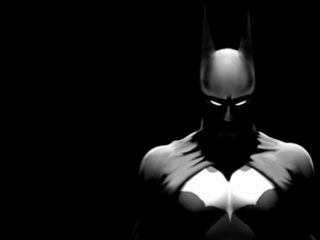
\includegraphics[width=.2\textwidth]{images/img.jpg}};
    \node (i4_4) [image, right of=i4_3, xshift=0.2\textwidth] {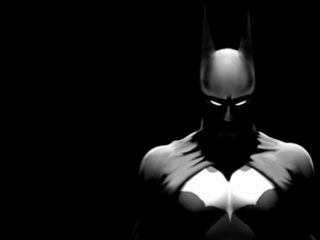
\includegraphics[width=.2\textwidth]{images/img.jpg}};
    \node (i4_5) [image, right of=i4_4, xshift=0.2\textwidth] {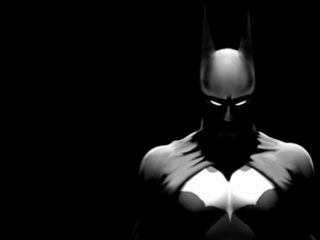
\includegraphics[width=.2\textwidth]{images/img.jpg}};

    \node (c5) [label, below of=c4, yshift=-0.2\textwidth] {micro-movement};
    \node (i5_1) [image, right of=c5, xshift=0.18\textwidth] {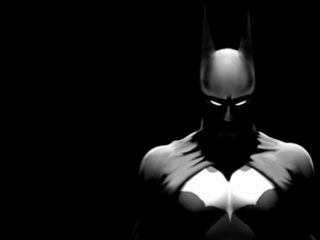
\includegraphics[width=.2\textwidth]{images/img.jpg}};
    \node (i5_2) [image, right of=i5_1, xshift=0.2\textwidth] {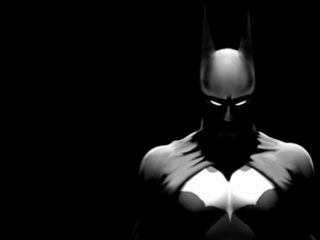
\includegraphics[width=.2\textwidth]{images/img.jpg}};
    \node (i5_3) [image, right of=i5_2, xshift=0.2\textwidth] {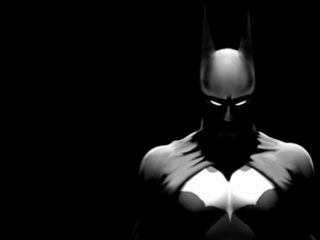
\includegraphics[width=.2\textwidth]{images/img.jpg}};
    \node (i5_4) [image, right of=i5_3, xshift=0.2\textwidth] {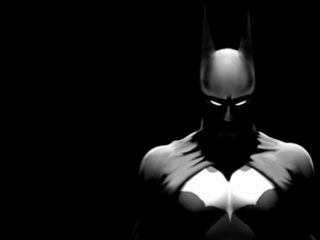
\includegraphics[width=.2\textwidth]{images/img.jpg}};
    \node (i5_5) [image, right of=i5_4, xshift=0.2\textwidth] {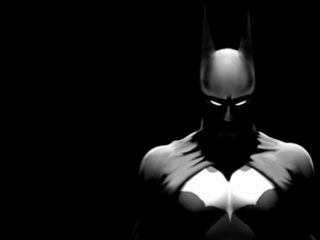
\includegraphics[width=.2\textwidth]{images/img.jpg}};

    \node (c6) [label, below of=c5, yshift=-0.2\textwidth] {rear};
    \node (i6_1) [image, right of=c6, xshift=0.18\textwidth] {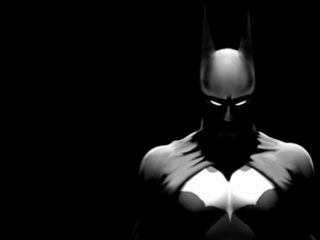
\includegraphics[width=.2\textwidth]{images/img.jpg}};
    \node (i6_2) [image, right of=i6_1, xshift=0.2\textwidth] {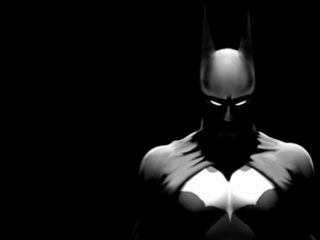
\includegraphics[width=.2\textwidth]{images/img.jpg}};
    \node (i6_3) [image, right of=i6_2, xshift=0.2\textwidth] {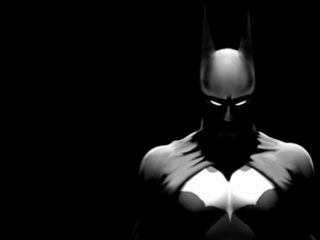
\includegraphics[width=.2\textwidth]{images/img.jpg}};
    \node (i6_4) [image, right of=i6_3, xshift=0.2\textwidth] {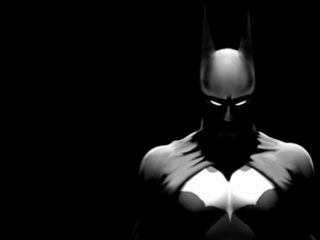
\includegraphics[width=.2\textwidth]{images/img.jpg}};
    \node (i6_5) [image, right of=i6_4, xshift=0.2\textwidth] {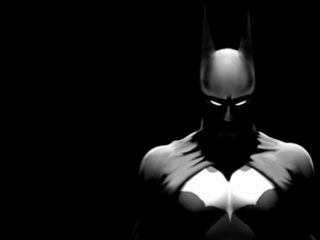
\includegraphics[width=.2\textwidth]{images/img.jpg}};

    \node (c7) [label, below of=c6, yshift=-0.2\textwidth] {rest};
    \node (i7_1) [image, right of=c7, xshift=0.18\textwidth] {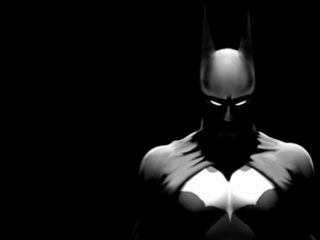
\includegraphics[width=.2\textwidth]{images/img.jpg}};
    \node (i7_2) [image, right of=i7_1, xshift=0.2\textwidth] {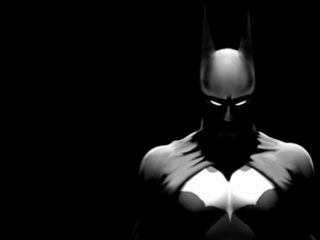
\includegraphics[width=.2\textwidth]{images/img.jpg}};
    \node (i7_3) [image, right of=i7_2, xshift=0.2\textwidth] {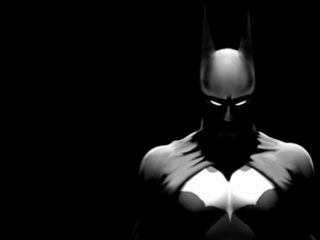
\includegraphics[width=.2\textwidth]{images/img.jpg}};
    \node (i7_4) [image, right of=i7_3, xshift=0.2\textwidth] {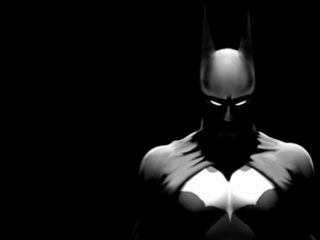
\includegraphics[width=.2\textwidth]{images/img.jpg}};
    \node (i7_5) [image, right of=i7_4, xshift=0.2\textwidth] {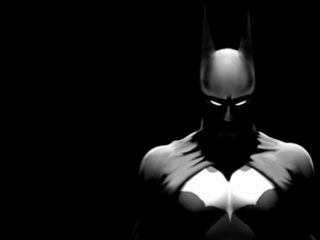
\includegraphics[width=.2\textwidth]{images/img.jpg}};

    \node (c8) [label, below of=c7, yshift=-0.2\textwidth] {walk};
    \node (i8_1) [image, right of=c8, xshift=0.18\textwidth] {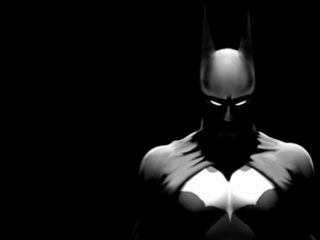
\includegraphics[width=.2\textwidth]{images/img.jpg}};
    \node (i8_2) [image, right of=i8_1, xshift=0.2\textwidth] {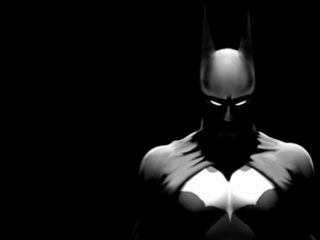
\includegraphics[width=.2\textwidth]{images/img.jpg}};
    \node (i8_3) [image, right of=i8_2, xshift=0.2\textwidth] {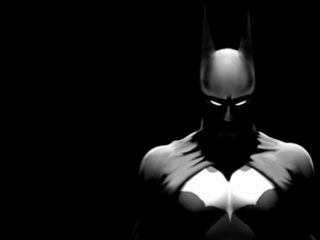
\includegraphics[width=.2\textwidth]{images/img.jpg}};
    \node (i8_4) [image, right of=i8_3, xshift=0.2\textwidth] {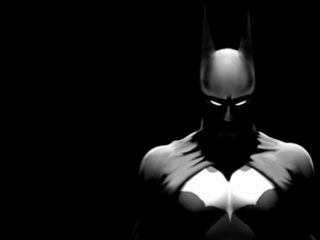
\includegraphics[width=.2\textwidth]{images/img.jpg}};
    \node (i8_5) [image, right of=i8_4, xshift=0.2\textwidth] {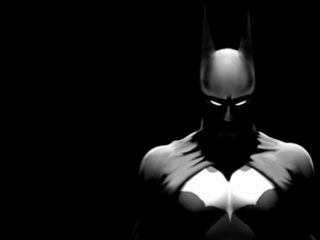
\includegraphics[width=.2\textwidth]{images/img.jpg}};

\end{tikzpicture}

\end{document}